\documentclass[12pt]{article}

\usepackage{sbc-template}
\usepackage{graphicx,url}
\usepackage[utf8]{inputenc}
\usepackage[brazil]{babel}
%\usepackage[latin1]{inputenc}
%\usepackage[T1]{fontenc}
\usepackage{graphicx}
\usepackage{svg}
\usepackage{minted}

\sloppy

\title{Treinamento de Modelos de Machine Learning para Detecção de Ransomware Baseado em Dataset Publico \\ Um Estudo de Caso de 4 Modelos}

\author{João Vítor Santa Brígida da Silva \inst{1}}
\address{
Programa de Pós-Graduação em Computação Aplicada (PPCA) \\ Universidade Federal do Pará (UFPA) -- Tucuruí -- PA -- Brasil
\email{joao.silva@castanhal.ufpa.br}
}

\begin{document}

\maketitle

\begin{abstract}
	
	Ransomware detection is a critical challenge for cybersecurity, requiring solutions that identify threats in real-time based on behavior. This work presents a case study focused on the training and evaluation of four Machine Learning models: BernoulliNB, Random Forest, Logistic Regression, and KNN. Using a dynamic analysis dataset with 1,524 samples (582 ransomware and 942 goodware), the methodology employed the Variance Threshold technique to reduce high dimensionality from 30,967 to 485 essential binary attributes, such as API calls and registry operations. The models were optimized via GridSearchCV, resulting in superior performance for Logistic Regression and Random Forest, both achieving an \textbf{F1-score above 96\%}. Additionally, the study explored model interpretability through native coefficients and the SHAP framework, identifying decisive behavioral patterns for threat classification.
\end{abstract}

\begin{resumo} 
	A detecção de ransomware representa um desafio crítico para a segurança cibernética, demandando soluções que identifiquem ameaças em tempo real com base em comportamento. Este trabalho apresenta um estudo de caso focado no treinamento e avaliação de quatro modelos de \textit{Machine Learning}: BernoulliNB, Random Forest, Logistic Regression e KNN. Utilizando um dataset de análise dinâmica com 1.524 amostras (582 ransomware e 942 \textit{goodwares}), a metodologia empregou a técnica de \textit{Variance Threshold} para reduzir a alta dimensionalidade de 30.967 para 485 atributos binários essenciais, como chamadas de API e operações de registro. Os modelos foram otimizados via \textit{GridSearchCV}, resultando em desempenhos superiores para a Regressão Logística e Random Forest, ambos com \textbf{F1-score acima de 96\%}. Adicionalmente, o estudo explorou a interpretabilidade dos modelos através de coeficientes nativos e do framework SHAP, identificando padrões comportamentais decisivos para a classificação das ameaças.
\end{resumo}


\section{Introdução} \label{sec:intro}

A detecção de ameaças cibernéticas, especificamente o ransomware, representa um desafio crescente para a segurança da informação, exigindo métodos eficazes para identificar comportamentos maliciosos em tempo real. Este trabalho apresenta um estudo de caso sobre o treinamento de quatro modelos de Machine Learning voltados para a detecção de ransomware, fundamentado em um dataset público consolidado na literatura.

A abordagem adotada prioriza a análise dinâmica, que consiste na execução de amostras em ambientes controlados, como o \cite{cuckoosandbox}. Diferente da análise estática, a análise dinâmica permite capturar o comportamento real do código em execução, mitigando técnicas de evasão comuns, como a ofuscação e a criptografia de binários. O dataset utilizado, disponibilizado por \cite{sgandurra2016}, compreende um total de 1.524 amostras, sendo 582 (38,19\%) de ransomware e 942 (61,81\%) de \textit{goodwares} (aplicações legítimas).

Um aspecto central deste estudo é a engenharia de atributos, fundamentada em 30.967 características binárias que representam a presença ou ausência de ações específicas durante a execução. Esses atributos estão organizados em sete categorias comportamentais críticas:
\begin{itemize}
	\item \textbf{API}: Chamadas de sistema;
	\item \textbf{REG}: Operações em chaves de registro do Windows;
	\item \textbf{FILES e FILES EXT}: Operações e extensões de arquivos;
	\item \textbf{DROP, DIR e STR}: Criação de arquivos, operações em diretórios e strings incorporadas.
\end{itemize}

O objetivo principal deste artigo é avaliar o desempenho dos algoritmos \textbf{BernoulliNB}, \textbf{Random Forest}, \textbf{Logistic Regression} e \textbf{KNN} na classificação dessas ameaças. Além da busca pela alta acurácia e otimização de hiperparâmetros via \textbf{GridSearchCV}, o trabalho dedica-se à interpretabilidade e explicabilidade dos modelos. Através de coeficientes nativos e do framework SHAP, busca-se compreender quais chamadas de API e operações de sistema são determinantes para a identificação de um ransomware.

\section{Materiais e Métodos} \label{sec:metodo}

Nesta seção, detalham-se os procedimentos e ferramentas utilizados para a obtenção e análise inicial dos dados que fundamentam este estudo.

\subsection{Descrição do Dataset e Coleta de Dados} \label{subsec:dataset}
A base de dados selecionada para este trabalho consiste em eventos de execução em sandbox (análise dinâmica), especificamente o dataset público disponibilizado por \cite{sgandurra2016}. Esta escolha justifica-se pelo fato de o dataset ser bem referenciado em estudos de segurança e inteligência artificial, servindo como base consolidada para a análise de comportamentos maliciosos \cite{caio2022}.

\subsubsection{A. Natureza e Origem dos Dados} \label{subsubsec:dataset-natureza}
Os dados foram gerados por meio da execução de amostras em um ambiente controlado utilizando a ferramenta \textit{Cuckoo Sandbox} \cite{cuckoosandbox}. Ao contrário da análise estática, a análise dinâmica permite capturar o comportamento real do código em execução, mitigando técnicas de evasão como ofuscação e criptografia de binários \cite{sgandurra2016}. O dataset é composto por um total de 1.524 amostras, divididas em:
\begin{itemize}
    \item \textbf{582 malwares (Ransomware):} Representando 38,19\% do total.
    \item \textbf{942 goodwares (Aplicações legítimas):} Representando 61,81\% do total.
\end{itemize}

As amostras de ransomware estão subdivididas em 11 famílias distintas, permitindo uma análise granular dos diferentes padrões de ataque \cite{sgandurra2016}. Entre as famílias presentes, destacam-se \textit{CryptLocker} (107 amostras), \textit{Locker} (97) e \textit{Reveton} (90), como é listado mais detalhadamente na tabela ~\ref{tab:dataset-stats}.

\subsubsection{B. Variáveis e Engenharia de Atributos (Features)} \label{subsubsec:dataset-variaveis}
O dataset original contém 30.967 atributos binários, que representam a presença (1) ou ausência (0) de uma determinada ação ou evento durante a execução\cite{sgandurra2016}.
Para este estudo foi incialmente desenvolvido um script em python (Figura ~\ref{fig:cod-dataset-stats}) para o levantamento estatístico inicial do dataset (mais detalhado na Tabela ~\ref{tab:dataset-stats}). Estes atributos estão organizados em sete categorias de comportamento:
\begin{itemize}
    \item \textbf{API:} Invocações de chamadas de sistema (\textit{API calls}).
    \item \textbf{DROP:} Extensões de arquivos criados (\textit{dropped}) durante a execução.
    \item \textbf{REG:} Operações em chaves de registro do Windows.
    \item \textbf{FILES:} Operações gerais de sistema de arquivos (leitura, escrita, deleção).
    \item \textbf{FILES\_EXT (EXT):} Extensões dos arquivos envolvidos nas operações de arquivo.
    \item \textbf{DIR:} Operações em diretórios (criação, enumeração).
    \item \textbf{STR:} Strings incorporadas no binário original.
\end{itemize}

\subsection{Estatísticas do Dataset} \label{subsec:dataset-stats}
A Tabela \ref{tab:dataset-stats} apresenta a distribuição detalhada das amostras de ransomware por família, conforme extraído do processamento dos dados brutos.
\begin{figure}[htbp]
	\centering
	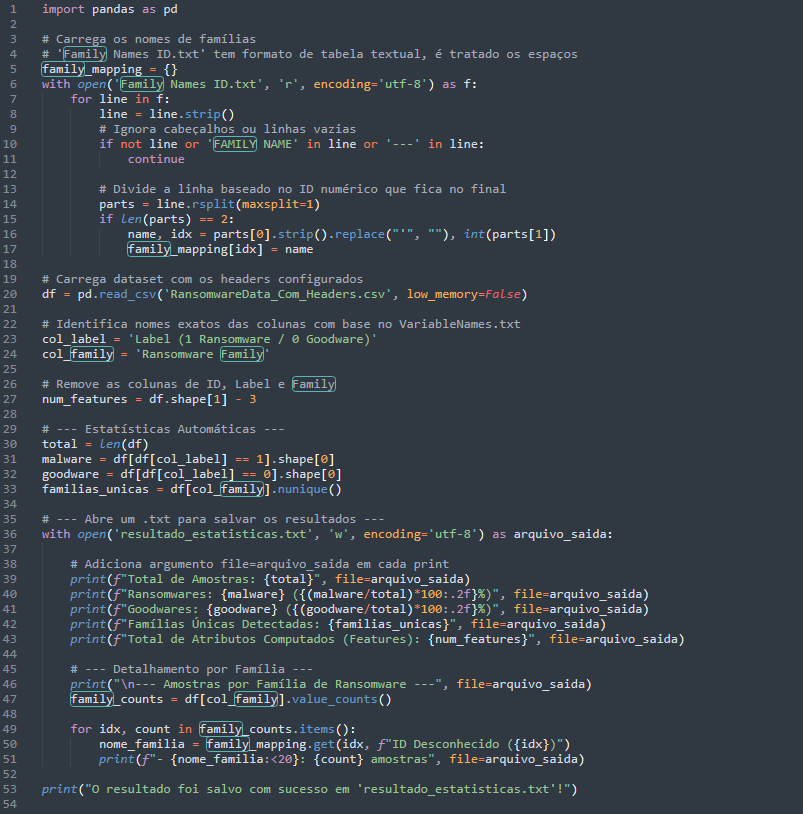
\includegraphics[width=.8\textwidth]{images/codigo_estatistica.png}
	\caption{Script Python para levantamento estatístico do dataset.}
	\label{fig:cod-dataset-stats}
\end{figure}

\begin{table}[htbp]
    \centering
    \caption{Visão Geral e Distribuição de Amostras do Dataset Sgandurra (2016).}
    \label{tab:dataset-stats}
    \begin{tabular}{|l|c|}
    \hline
    \textbf{Métrica} & \textbf{Valor / Quantidade} \\ \hline
    Total de Amostras & 1.524 \\ \hline
    Ransomwares & 582 (38.19\%) \\ \hline
    Goodwares & 942 (61.81\%) \\ \hline
    Famílias Únicas Detectadas & 11 \\ \hline
    Total de Atributos Computados (Features) & 30.967 \\ \hline
    \hline
    \multicolumn{2}{|c|}{\textbf{Amostras por Família de Ransomware}} \\ \hline
    Goodware & 942 \\ \hline
    CryptLocker & 107 \\ \hline
    Locker & 97 \\ \hline
    Reveton & 90 \\ \hline
    Kovter & 64 \\ \hline
    MATSNU & 59 \\ \hline
    Critroni & 50 \\ \hline
    CryptoWall & 46 \\ \hline
    Trojan-Ransom & 34 \\ \hline
    KOLLAH & 25 \\ \hline
    TeslaCrypt & 6 \\ \hline
    PGPCODER & 4 \\ \hline
    \end{tabular}
\end{table}

%\begin{minted}{python}
%def ola_mundo():
%    print("Olá, LaTeX!")
%\end{minted}

\section{Pre-Processamento} \label{sec:preproc}

Este capítulo detalha as etapas de preparação do conjunto de dados, abordando a limpeza de dados, a seleção de atributos e a fundamentação teórica que sustenta as escolhas técnicas realizadas para otimizar o treinamento dos modelos de detecção de ransomware.

\subsection{Limpeza de Dados e Seleção de Atributos via Variance Threshold} \label{subsec:limpezadados}

O conjunto de dados original apresentava uma alta dimensionalidade, com um total de 30.967 atributos comportamentais. No entanto, observou-se que a vasta maioria desses atributos (98,46\%) possuía uma baixíssima densidade de informação, apresentando entre 0 e 50 eventos em um universo de 1.524 amostras. Para reduzir este problema de esparsidade e minimizar o custo computacional, aplicou-se a técnica de seleção de atributos \textit{Variance Threshold (VT)}.

O VT é um método do tipo filtro não supervisionado que remove recursos cuja variância não atinge um limite especificado \cite{kuhn2013applied}. Dado que o \textit{dataset} é composto por variáveis binárias (booleanas), a variância é calculada com base no ensaio de Bernoulli, conforme a Equação ~\ref{eq:variancia}:
\begin{equation} \label{eq:variancia} 
	Var[X] = p(1 - p) 
\end{equation}
\begin{center}
	\textbf{Equação para o cálculo da variância}.
\end{center}

Onde $p$ representa a probabilidade de sucesso (parâmetro de probabilidade de Bernoulli), que define o percentual do limite de corte \cite{scikit-learn}. Neste trabalho, utilizou-se um limite de variância de 97\% ($p = 0.97$). Na prática, isso resultou na exclusão de todas as colunas onde o mesmo valor (0 ou 1) se repetia em mais de 97\% das amostras, ou seja, atributos com 45 ou menos ocorrências de um dos valores foram descartados por não serem considerados cruciais. Esta etapa reduziu drasticamente o número de atributos de 30.923 para 485, permitindo uma análise mais focada em características realmente discriminantes.

\subsection{Normalização e Mapeamento de Atributos} \label{subsec:normalizacao}

Quanto à normalização, o conjunto de dados já se encontrava modelado em formato binário, onde o valor '1' indica a presença de uma operação ou evento e '0' indica sua ausência. Devido a essa natureza booleana intrínseca, não foi necessária a aplicação de técnicas de reescalonamento numérico adicionais.

Uma tarefa essencial de pré-processamento foi a atribuição de nomes às \textit{features}. Como o \textit{dataset} público original não possuía cabeçalhos nas colunas, foi realizado o mapeamento técnico de cada atributo utilizando um arquivo de metadados separado. Esta ação foi fundamental para garantir a interpretabilidade dos resultados, permitindo identificar quais chamadas de API ou operações de registro são mais frequentes em amostras de ransomware em comparação a \textit{goodwares}.

\subsection{Fundamentação Teórica} \label{subsec:fundamentacao}

A escolha pelo \textit{Variance Threshold} justifica-se por ser uma abordagem não supervisionada de filtro. Diferente de métodos supervisionados, o VT pode ser aplicado ao conjunto de dados global antes da estratégia de validação cruzada (\textit{Cross-validation}), garantindo que os mesmos atributos sejam mantidos em todas as iterações de treino e teste sem o risco de \textit{overfitting} \cite{james2013introduction}. Além disso, como um método de filtragem, o VT preserva o significado original das variáveis, o que é vital para a análise comportamental de \textit{malwares} \cite{scikit-learn}. 

A literatura de aprendizado de máquina sustenta que o uso de distribuições de Bernoulli para o cálculo de variância em dados binários é a abordagem estatística correta para identificar recursos com baixa variabilidade \cite{hastie2009elements}. Estudos anteriores utilizando este mesmo \textit{dataset} demonstraram que a redução de dimensionalidade para cerca de 400-500 atributos mantém ou até melhora a acurácia dos classificadores, validando a eficácia do limite de 97\% adotado \cite{sgandurra2016, caio2022}.

\section{Treinamento dos Modelos de Machine Learning} \label{sec:treinamento}

Este capítulo descreve o processo de treinamento e otimização dos modelos de \textit{Machine Learning} utilizados para a detecção de \textit{ransomware}. O objetivo principal é classificar o \textit{dataset} entre as categorias \textit{goodware} e \textit{malware}, empregando técnicas de aprendizado supervisionado utilizando  Python, com o auxílio da biblioteca \textit{Scikit-learn}.

\subsection{Seleção de Modelos e Hiperparâmetros}

Para este estudo, optou-se pela abordagem de \textbf{aprendizado supervisionado}, sendo selecionados quatro algoritmos classificadores distintos para avaliação:

\begin{itemize}
    \item \textbf{BernoulliNB:} Um classificador Naive Bayes adequado para dados discretos. Os hiperparâmetros pesquisados incluíram \textit{alpha}, \textit{binarize} e \textit{fit\_prior}.
    \item \textbf{Random Forest:} Um método de aprendizado de conjunto (\textit{ensemble learning}). Foram analisados os parâmetros \textit{class\_weight}, \textit{criterion}, \textit{max\_depth} e \textit{n\_estimators}.
    \item \textbf{Logistic Regression:} Utilizado para classificação linear. A pesquisa de hiperparâmetros focou em \textit{C}, \textit{max\_iter}, \textit{penalty} e \textit{solver}.
    \item \textbf{KNeighborsClassifier (KNN):} Baseado na proximidade de vizinhos. Os parâmetros ajustados foram \textit{metric}, \textit{n\_neighbors} e \textit{weights}.
\end{itemize}

\subsection{Otimização com GridSearchCV} \label{subsec:grid}

Para maximizar o desempenho dos modelos, especificamente a métrica \textbf{F1-score}, foi realizado o ajuste de hiperparâmetros utilizando a técnica de \textit{GridSearchCV} com validação cruzada, utilizando \textbf{Folds = 5} e \textbf{Repetições = 10}. Este processo permitiu identificar a melhor configuração para cada modelo, conforme detalhado na Tabela \ref{tab:melhores_parametros}.

\begin{table}[htbp]
\centering
\caption{Melhores Hiperparâmetros Identificados via GridSearchCV}
\label{tab:melhores_parametros}
\begin{tabular}{|l|p{10cm}|}
\hline
\textbf{Modelo} & \textbf{Melhores Parâmetros Configurativos} \\ \hline
BernoulliNB & \{'alpha': 0.001, 'binarize': None, 'fit\_prior': False\} \\ \hline
KNN & \{'metric': 'manhattan', 'n\_neighbors': 3, 'weights': 'distance'\} \\ \hline
Logistic Regression & \{'C': 1.0, 'max\_iter': 1000, 'penalty': 'l1', 'solver': 'saga'\} \\ \hline
Random Forest & \{'class\_weight': 'None', 'criterion': 'entropy', 'max\_depth': 20, 'n\_estimators': 100\} \\ \hline
\end{tabular}
\end{table}

\subsection{Resultados e Discussão} \label{subsec:resultados}

Após a identificação dos melhores hiperparâmetros, os modelos foram reavaliados. A Tabela \ref{tab:comparativo_modelos} apresenta os resultados comparativos de desempenho, considerando as métricas de Acurácia, Precisão, \textit{Recall} e F1-score, acompanhadas de seus respectivos intervalos de confiança de 95\%.

\begin{table}[htbp]
	\centering
	\caption{Comparativo de Desempenho dos Modelos Otimizados}
	\label{tab:comparativo_modelos}
	\begin{tabular}{|l|c|c|c|c|}
		\hline
		\textbf{Modelo} & \textbf{Acurácia (\%)} & \textbf{Precisão (\%)} & \textbf{Recall (\%)} & \textbf{F1-score (\%)} \\ \hline
		BernoulliNB & 82,09 $\pm$ 0,57 & 71,77 $\pm$ 0,78 & 87,80 $\pm$ 0,79 & 78,94 $\pm$ 0,62 \\ \hline
		KNN & 95,58 $\pm$ 0,23 & 93,99 $\pm$ 0,62 & 94,57 $\pm$ 0,54 & 94,24 $\pm$ 0,29 \\ \hline
		Logistic Regression & 97,69 $\pm$ 0,23 & 97,35 $\pm$ 0,37 & 96,60 $\pm$ 0,43 & 96,96 $\pm$ 0,30 \\ \hline
		Random Forest & 97,82 $\pm$ 0,20 & 97,58 $\pm$ 0,36 & 96,70 $\pm$ 0,44 & 97,12 $\pm$ 0,26 \\ \hline
	\end{tabular}
\end{table}

Os resultados demonstram que os modelos de \textbf{Logistic Regression} e \textbf{Random Forest} apresentaram os melhores desempenhos gerais, ambos superando a marca de 96\% em F1-score após a otimização. O modelo KNN também apresentou um desempenho sólido (92,59\% F1-score), enquanto o BernoulliNB, embora eficaz, obteve métricas inferiores aos demais classificadores testados.


\section{Interpretando o Modelo e Análise de Influência das Features} 
\label{sec:avaliacao}

Este capítulo descreve o processo de interpretação dos resultados obtidos pelo modelo selecionado para a detecção de malwares. A interpretabilidade é um componente crítico em segurança cibernética, pois permite não apenas a classificação, mas a compreensão dos comportamentos que levam o modelo a identificar uma ameaça.

\subsection{Seleção e Treinamento do Modelo} \label{subsec:treinamento}

Com base em experimentos prévios, o modelo de \textbf{Regressão Logística} foi o escolhido para a análise final. Esta decisão fundamentou-se no fato de o modelo apresentar resultados de acurácia próximos aos do Random Forest, porém com um desempenho de processamento e eficiência computacional consideravelmente superiores. O treinamento foi realizado utilizando os seguintes hiperparâmetros otimizados:

\begin{itemize}
    \item Penalidade: $L1$ Lasso (Least Absolute Shrinkage and Selection Operator);
    \item Parâmetro de Regularização ($C$): $1.0$;
    \item Solucionador: \textit{saga};
    \item Máximo de iterações: $1000$.
\end{itemize}

\subsection{Cálculo Nativo de Importância (Coeficientes)} \label{subsec:calcnativo}

A Regressão Logística, por ser um modelo linear, permite uma interpretação direta através de seus coeficientes \cite{hosmer2013applied}. Cada variável de entrada (feature) recebe um peso que representa sua contribuição para o log-odds da classe alvo.

\begin{figure}[htbp]
    \centering
    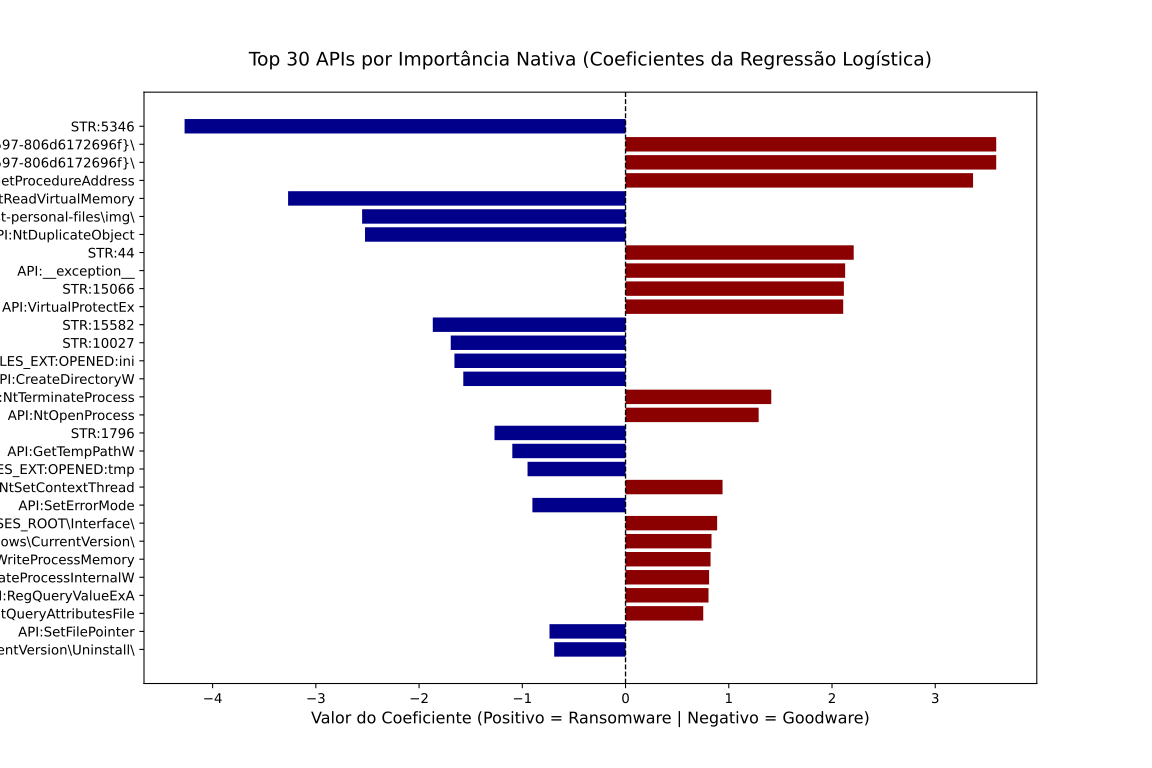
\includegraphics[width=0.8\textwidth]{images/calcnativo_regressao.png}
    \caption{Grafico do Calculo Nativo do modelo Logistic Regression em seus melhores parametros.}
    \label{fig:calcnativo-regressao}
\end{figure}

A Figura ~\ref{fig:calcnativo-regressao} apresenta o \textit{Top 30 APIs por Importância Nativa}. No gráfico:
\begin{itemize}
    \item \textbf{Coeficientes Positivos (Vermelho):} Indicam que a presença ou alta frequência da API aumenta a probabilidade de a amostra ser classificada como \textit{Ransomware}. Destacam-se APIs relacionadas a manipulação de strings e acesso a registros.
    \item \textbf{Coeficientes Negativos (Azul):} Indicam uma associação com \textit{Goodware}. A API \texttt{STR:5346} e \texttt{API:NtReadVirtualMemory} apresentam os maiores pesos negativos, sugerindo que são características predominantes em softwares legítimos no dataset analisado.
\end{itemize}

\subsection{Análise de Explicabilidade com SHAP} \label{subsec:shap}

Para aprofundar a compreensão sobre a influência das features, utilizamos o framework SHAP (\textit{SHapley Additive exPlanations}), fundamentado na teoria dos jogos cooperativos \cite{lundberg2017unified}. O SHAP oferece uma visão mais granular do que os coeficientes globais, permitindo observar o impacto de cada feature em cada predição individual.

\subsubsection{Beeswarm Plot} \label{subsubsec:beeswarm}

O gráfico \textit{Beeswarm} (Figura ~\ref{fig:beeswarm}) fornece uma visão geral do impacto das top 30 APIs no modelo.

\begin{figure}[htbp]
    \centering
    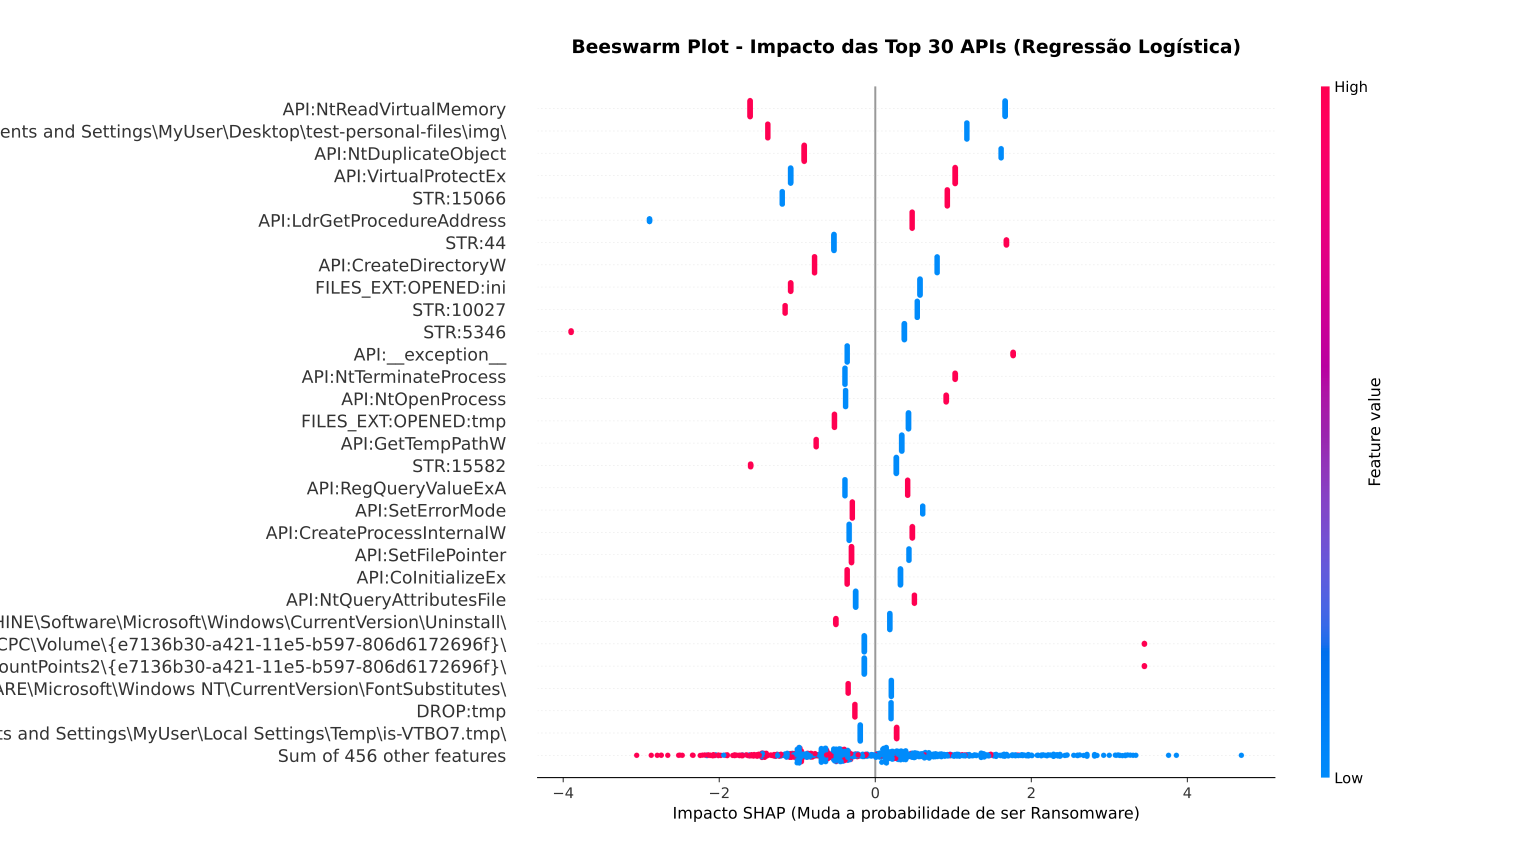
\includegraphics[width=0.8\textwidth]{images/shap_lregression_beeswarm.png}
    \caption{Grafico SHAP Beeswarm com o modelo Logistic Regression em seus melhores parametros.}
    \label{fig:beeswarm}
\end{figure}

\begin{itemize}
    \item O eixo horizontal representa o \textbf{Impacto SHAP}: valores à direita aumentam a probabilidade de \textit{Ransomware}, enquanto à esquerda diminuem.
    \item A cor indica o valor da feature (Vermelho para alto, Azul para baixo). 
    \item Observa-se que para a API \texttt{NtReadVirtualMemory}, valores baixos (azul) têm um impacto negativo forte, corroborando o gráfico de coeficientes nativos, enquanto para outras APIs, a dispersão dos pontos revela comportamentos não lineares capturados pelo modelo.
\end{itemize}

\subsubsection{Decision Plot} \label{subsubsec:decisionplot}

O grafico \textit{Decision Plot} Figura ~\ref{fig:bdecision} ilustra o caminho de decisão para 50 amostras específicas.

\begin{figure}[htbp]
    \centering
    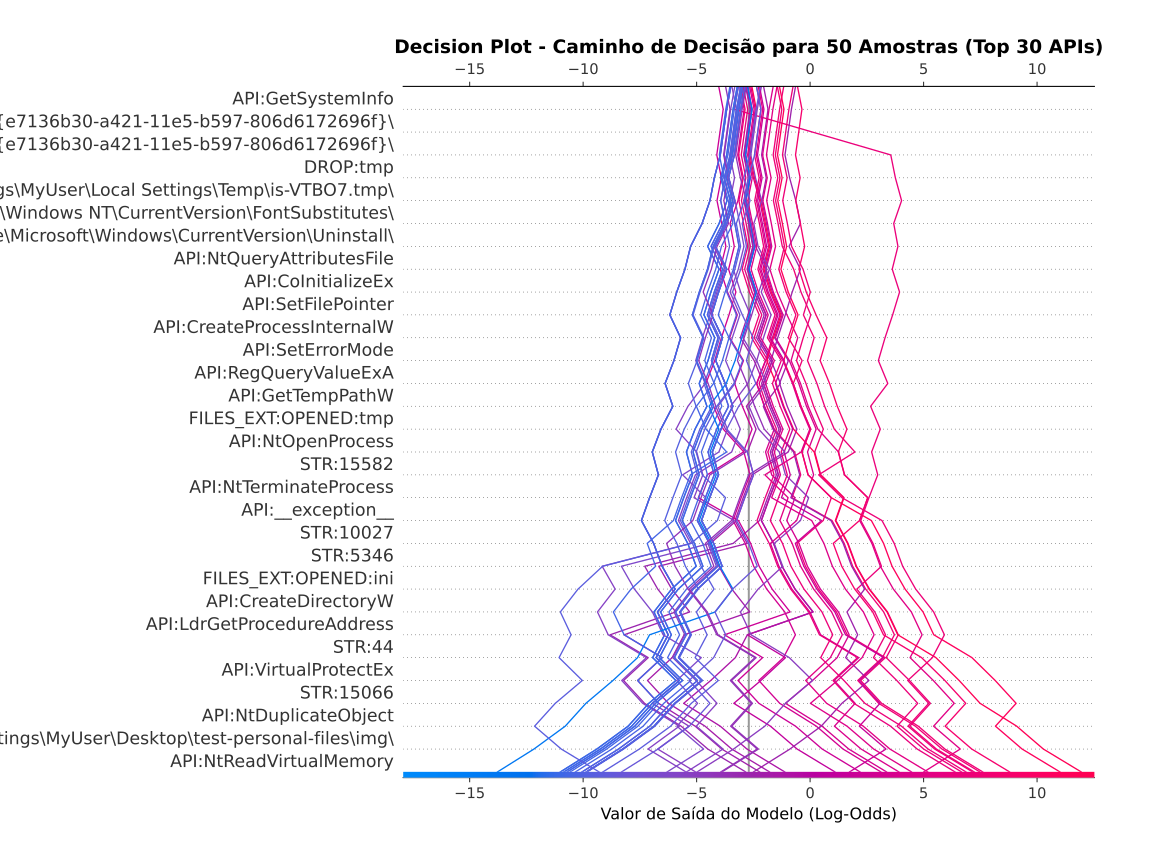
\includegraphics[width=0.8\textwidth]{images/shap_lregression_bdecision.png}
    \caption{Grafico SHAP Decision Plot com o modelo Logistic Regression em seus melhores parametros.}
    \label{fig:bdecision}
\end{figure}

\begin{itemize}
    \item O gráfico mostra como as predições individuais evoluem a partir de um valor base (valor médio esperado) conforme cada API é considerada.
    \item As linhas que convergem para a direita (em rosa) representam amostras com alta probabilidade de serem maliciosas, enquanto as que tendem para a esquerda (em azul) são classificadas como benignas.
    \item Este gráfico é essencial para identificar quais combinações de APIs são determinantes para a classificação final do modelo em casos específicos de \textit{log-odds}.
\end{itemize}

\section{Conclusão} \label{sec:conclu}

Este estudo realizou uma análise comparativa de quatro modelos de \textit{Machine Learning} para a detecção de ransomware, utilizando um dataset baseado em análise dinâmica com 1.524 amostras. Os resultados demonstram a viabilidade e a eficácia de utilizar o comportamento em execução para diferenciar códigos maliciosos de aplicações legítimas (\textit{goodwares}).

A etapa de pré-processamento, especificamente a aplicação da técnica de \textit{Variance Threshold}, mostrou-se fundamental. A redução drástica da dimensionalidade de 30.967 para 485 atributos não apenas diminuiu o custo computacional, mas manteve a capacidade discriminante necessária para o treinamento dos modelos. Entre os algoritmos avaliados, a Regressão Logística e o Random Forest destacaram-se com desempenhos superiores, ambos alcançando um F1-score acima de 96\%.

A escolha da Regressão Logística para a análise final foi justificada por seu equilíbrio entre alta acurácia e eficiência computacional. Além da detecção, este trabalho contribuiu para a explicabilidade do modelo ao utilizar coeficientes nativos e o framework SHAP. Essa análise permitiu identificar que chamadas de API específicas e operações de sistema, como as relacionadas à manipulação de strings e acesso a registros, são indicadores críticos de comportamento de ransomware no dataset estudado.

Em suma, a metodologia adotada prova que a combinação de engenharia de atributos focada em comportamento e modelos de aprendizado supervisionado é uma abordagem robusta para enfrentar as ameaças cibernéticas modernas. Como trabalhos futuros, sugere-se a expansão do dataset para incluir famílias de ransomware mais recentes e a exploração de métodos de aprendizado profundo (\textit{Deep Learning}) para capturar sequências temporais de chamadas de sistema.


\bibliographystyle{sbc}
\bibliography{referencias}

\end{document}
